% !TEX root = ../main.tex
\chapter[MÔI TRƯỜNG MÔ PHỎNG VÀ BỘ BỐI CẢNH NHIỆM VỤ]{MÔI TRƯỜNG MÔ PHỎNG\\VÀ BỘ BỐI CẢNH NHIỆM VỤ}
\label{chap:task-suite}

Chương này mô tả môi trường mô phỏng, cách bố trí bàn làm việc theo tầm với của robot và người, mô hình người, năm nhiệm vụ thuộc ba vai tương tác, và quy trình sinh dữ liệu trình diễn. Đây là nền tảng chung cho mọi thí nghiệm ở các chương sau.

\section{Môi trường mô phỏng}
\label{sec:sim}

Môi trường được xây dựng trên MuJoCo~\cite{todorov2012mujoco}, gồm các thành phần sau:
\begin{itemize}
  \item \textbf{Robot.} Tay máy UR3e sáu bậc tự do gắn tay kẹp SusGrip, đặt cạnh một bàn đứng cao 0,85~m. Hệ tọa độ gốc đặt tại đế robot: trục $+X$ hướng ra phía trước robot, $+Y$ sang trái robot, $+Z$ hướng lên.
  \item \textbf{Bộ điều khiển khớp.} Bộ điều khiển servo khớp được tăng hệ số khuếch đại ($k_p = 2000$, $k_v = 100$) để tay máy bám điểm đặt chặt chẽ.
  \item \textbf{Gắp có hỗ trợ.} Vì ngón kẹp SusGrip đi theo cung tròn khi đóng, việc gắp thuần ma sát trong mô phỏng không ổn định. Môi trường vì vậy dùng cơ chế \emph{gắp có hỗ trợ} tương tự iGibson~2.0~\cite{li2021igibson}: vật chỉ được gắn vào tay kẹp khi cả hai ngón chạm vật về mặt vật lý trong lúc kẹp đang đóng, và được nhả ngay khi kẹp mở.
\end{itemize}

\paragraph{Quan sát.} Chính sách nhận ba ảnh RGB độ phân giải $256\times192$ cùng một vector trạng thái 10 chiều (6 góc khớp, độ mở tay kẹp, vị trí điểm công cụ). Ba camera gồm (Hình~\ref{fig:cameras}):
\begin{itemize}
  \item camera \texttt{high} đặt ở mép bàn đối diện người, cao 1,5~m, thấy mặt và tay người trong mọi tư thế;
  \item camera \texttt{top} nhìn từ trên xuống cụm ô vật, hơi nghiêng để cánh tay robot lúc nghỉ không che các ô;
  \item camera \texttt{wrist} gắn cạnh tay kẹp theo kiểu \emph{eye-in-hand} của robosuite~\cite{zhu2020robosuite}.
\end{itemize}

\begin{figure}[htbp]
  \centering
  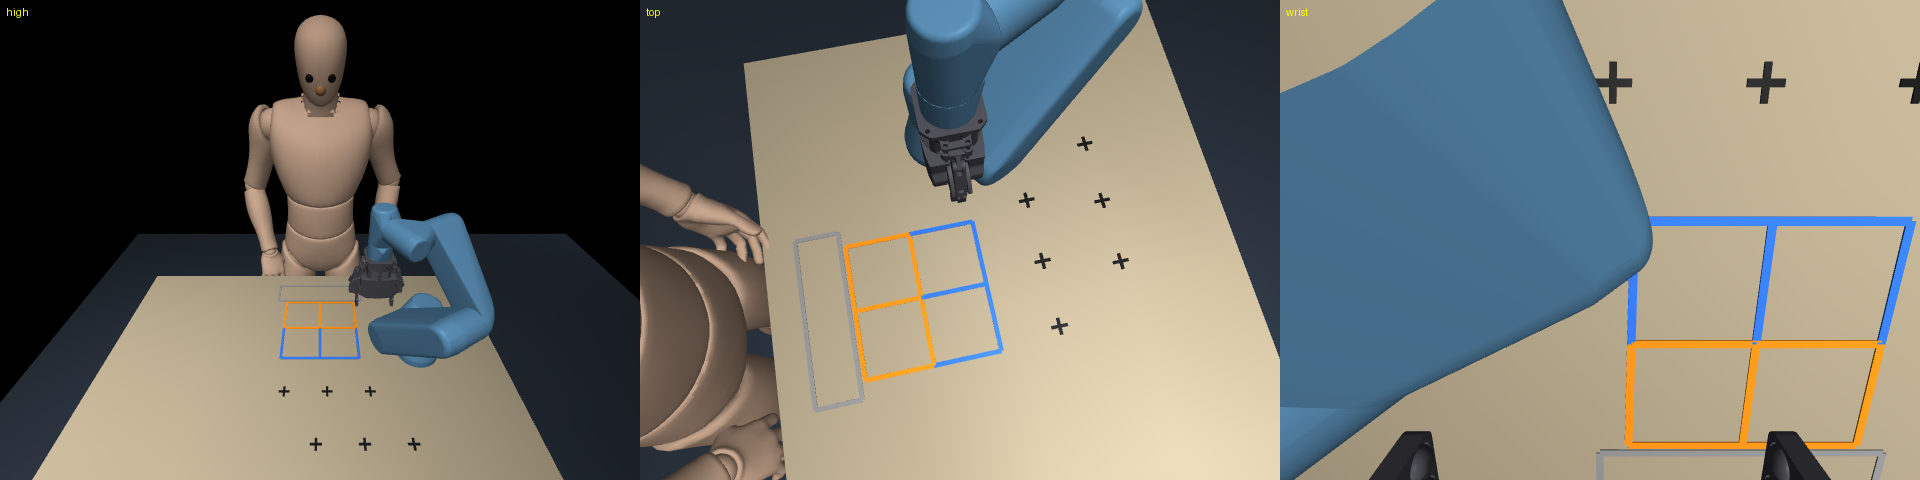
\includegraphics[width=\textwidth]{cameras}
  \caption{Ba góc camera của chính sách: \texttt{high} (trái), \texttt{top} (giữa) và \texttt{wrist} (phải).}
  \label{fig:cameras}
\end{figure}

\section{Bố trí bàn làm việc theo tầm với}
\label{sec:layout}

Người đứng ở mép bàn bên phải robot theo bố trí chéo $90^\circ$, lệch sang bên 0,30~m so với đế robot. Bàn được chia thành các vùng theo khả năng với tới. Tính từ phía người ra xa (Hình~\ref{fig:layout}):
\begin{itemize}
  \item \textbf{Vùng U} (chỉ người với tới): một dải $30\times8$~cm ngay trước người. Nửa phải là chỗ để hai khối mà người tự lấy trong nhiệm vụ T3; nửa trái (\texttt{U\_cup}) là chỗ robot đặt cốc.
  \item \textbf{Hàng H} (vùng chung): hai vùng trao vật H1, H2, nơi lòng bàn tay người nhận vật ở độ cao 15~cm trên mặt bàn.
  \item \textbf{Hàng P} (vùng chung): hai vùng đặt vật P1, P2.
  \item \textbf{Vùng robot}: hai hàng ô vật thẳng, mỗi hàng ba ô cách nhau 12~cm. Hàng gần là S4--S6, hàng xa là S1--S3, hai hàng lệch nhau 3~cm.
\end{itemize}

Bố trí được kiểm tra tự động theo các tiêu chí sau:
\begin{itemize}
  \item mọi vị trí robot cần chạm tới nằm trong bán kính hiệu dụng $R_\text{eff} = 0{,}40$~m, và robot gắp thành công 5/5 lần ở mọi vị trí;
  \item người với tới mọi vùng H, U và chỉ tới mọi ô P, S với độ nghiêng lưng không quá $30^\circ$;
  \item tia chỉ tay tới hai ô S bất kỳ lệch nhau ít nhất $5^\circ$, để mục tiêu của cử chỉ chỉ tay luôn phân biệt được về hình học.
\end{itemize}

\begin{figure}[htbp]
  \centering
  \begin{subfigure}{0.49\textwidth}
    \centering
    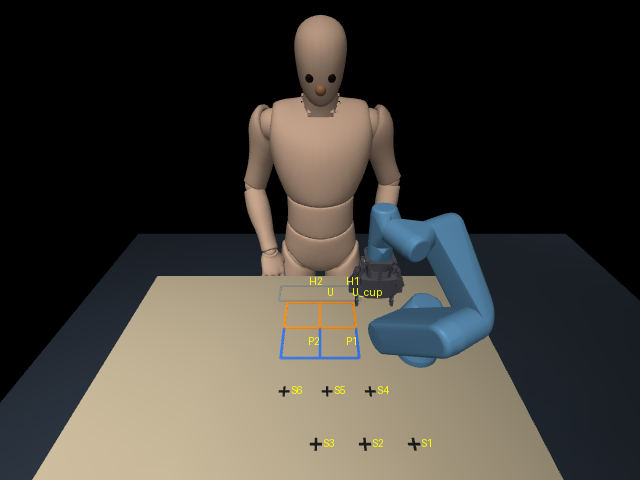
\includegraphics[width=\linewidth]{scene_overview}
    \caption{}
  \end{subfigure}\hfill
  \begin{subfigure}{0.49\textwidth}
    \centering
    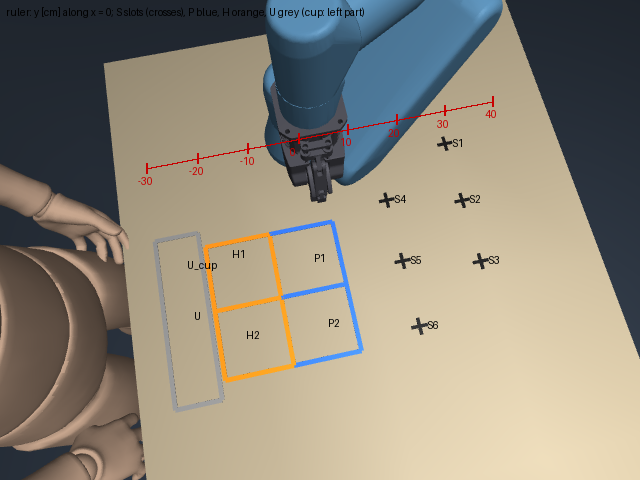
\includegraphics[width=\linewidth]{layout_top}
    \caption{}
  \end{subfigure}
  \caption{Bố trí bàn làm việc: (a) toàn cảnh từ camera \texttt{high}; (b) nhìn từ trên xuống với các ô vật S1--S6 (dấu chữ thập), vùng đặt P (xanh), vùng trao vật H (cam) và vùng người U (xám).}
  \label{fig:layout}
\end{figure}

\paragraph{Bộ vật.} Bộ vật gồm:
\begin{itemize}
  \item ba khối lập phương 4~cm màu đỏ (B1), xanh dương (B2) và vàng (B3);
  \item khối B1$'$ giống hệt B1, dùng để tạo tình huống mơ hồ mà chỉ cử chỉ mới phân biệt được;
  \item hai cốc trắng giống hệt nhau C1, C2 và một cốc xanh lá C3.
\end{itemize}
Mỗi episode đặt 3--4 vật trên bàn (riêng T4 chỉ có 1 khối).

\section{Mô hình người}
\label{sec:human}

Người trong mô phỏng là ma-nơ-canh của HY-Motion~1.0~\cite{wen2025hymotion}, dùng khung xương SMPL-H~\cite{romero2017mano}, được tách thành các đoạn cứng. Hành vi của người được \emph{lập trình sẵn} và tất định theo seed:
\begin{itemize}
  \item \textbf{Quỹ đạo.} Chỉ lòng bàn tay được điều khiển theo quỹ đạo min-jerk~\cite{flash1985minjerk}. Toàn thân được suy ra bằng động học ngược hai khâu cho cánh tay chủ động; thân người cúi ở eo vừa đủ để với tới.
  \item \textbf{Hình bàn tay.} Bàn tay có bốn hình cơ bản (tự nhiên, chỉ, nắm, ngửa đón) cùng các hình trung gian, nên ngón tay chuyển dáng mượt trong khoảng 0,2~s.
  \item \textbf{Chỉ tay.} Khi chỉ tay, cổ tay được ngắm sao cho tia ngón trỏ đi qua đúng mục tiêu, sai lệch dưới 2~cm, và cử chỉ được giữ 1,8--2,5~s (Hình~\ref{fig:human-poses}).
  \item \textbf{Va chạm.} Hình học người chỉ dùng để hiển thị. Va chạm và vi phạm khoảng cách an toàn được đo bằng khoảng cách tới các khối proxy ẩn (lòng bàn tay, cẳng tay, cánh tay trên, thân, đầu).
\end{itemize}

Việc người không phản ứng với robot là một giới hạn có chủ đích. Nhờ đó chuyển động của người \emph{giống hệt nhau} giữa các mô hình được so sánh, giống cách HRIBench cố định lịch xuất hiện của người~\cite{liu2026hribench}. Đây cũng là điều kiện để nguồn ý định \emph{hindsight}, vốn biết trước tương lai, được định nghĩa một cách hợp lệ.

\begin{figure}[htbp]
  \centering
  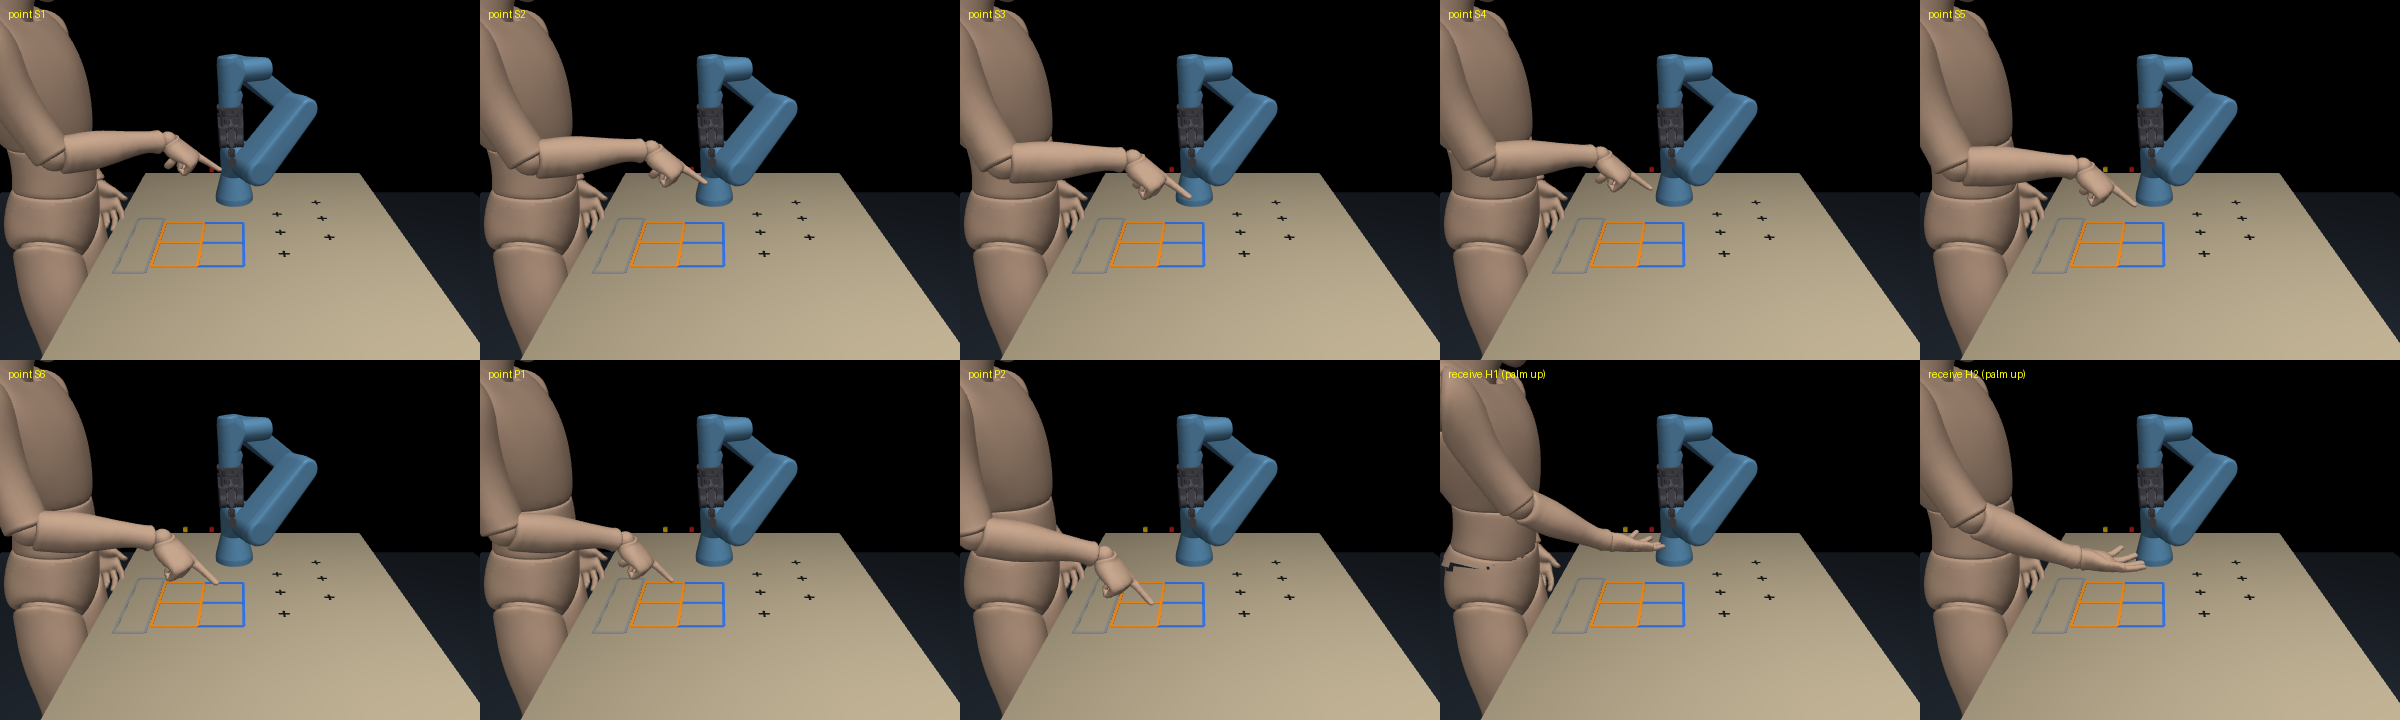
\includegraphics[width=\textwidth]{human_poses}
  \caption{Các cử chỉ của người trong mô phỏng: chỉ tới sáu ô vật S1--S6 và hai vùng đặt P1, P2, và ngửa lòng bàn tay nhận vật ở hai vùng H1, H2.}
  \label{fig:human-poses}
\end{figure}

\section{Bộ bối cảnh nhiệm vụ}
\label{sec:tasks}

Bộ nhiệm vụ gồm năm nhiệm vụ T1--T5 và một biến thể âm T4-neg, thuộc ba vai tương tác như HRIBench~\cite{liu2026hribench}. Bảng~\ref{tab:tasks} tóm tắt các nhiệm vụ.

\begin{table}[htbp]
  \centering
  \caption{Bộ bối cảnh nhiệm vụ.}
  \label{tab:tasks}
  \small
  \begin{tabularx}{\textwidth}{@{}l l X X@{}}
    \toprule
    \textbf{Nhiệm vụ} & \textbf{Vai} & \textbf{Hành vi của người} & \textbf{Robot cần làm / thành công khi} \\
    \midrule
    T1 gắp -- đặt & Instructor & Chỉ vào khối mục tiêu, rồi chỉ vào vùng đặt P & Gắp đúng khối, đặt vào đúng vùng P, về tư thế nghỉ; không chạm vật khác \\
    \addlinespace
    T2 trao vật & Collaborator & Chỉ vào vật, rồi ngửa tay ở một vùng H theo một trong ba thời điểm: sớm, đúng lúc, muộn & Mang đúng vật tới tay đang chờ, giữ yên, chỉ nhả khi người đã cầm \\
    \addlinespace
    T3 hỗ trợ & Collaborator & Không chỉ tay; tự lấy một trong hai khối ở U, mỗi khối gắn với một cốc & Đoán từ việc người với tới khối nào để mang đúng cốc tới \texttt{U\_cup} kịp lúc \\
    \addlinespace
    T4 xâm nhập & Intruder & Đưa tay vào vùng robot ở một trong ba pha (tiến tới vật, mang vật, sắp đặt), giữ 1, 2 hoặc 4~s & Tự gắp -- đặt một khối; dừng khi tay ở trong vùng, tiếp tục đúng chỗ đang dở, không va chạm \\
    \addlinespace
    T4-neg & Intruder & Tay đi gần nhưng ở ngoài vùng robot & Không được dừng không cần thiết \\
    \addlinespace
    T5 đổi ý & theo T1/T2/T3 & Ra hiệu mục tiêu cũ, rút tay, rồi ra hiệu mục tiêu mới; sớm hoặc muộn, luôn trước khi robot gắp & Hoàn thành nhiệm vụ gốc với mục tiêu mới, không chạm vật cũ \\
    \bottomrule
  \end{tabularx}
\end{table}

Mỗi nhiệm vụ kiểm tra một khía cạnh khác nhau của thông tin ý định:
\begin{itemize}
  \item T1 cần thông tin \emph{không gian} (vật nào, đặt ở đâu); trong một phần ba số episode có hai khối giống hệt nhau, nên chỉ cử chỉ mới phân biệt được.
  \item T2 cần thông tin \emph{thời gian}: robot phải tới vùng H đúng lúc tay người sẵn sàng.
  \item T3 là một ``quy trình đã học'': mục tiêu được suy ra từ chuyển động vươn tay chứ không từ cử chỉ chỉ dẫn, nên kiểm tra khả năng đoán sớm.
  \item T4 và T4-neg kiểm tra phản ứng an toàn và khả năng phân biệt xâm nhập thật với chuyển động lân cận vô hại.
  \item T5 kiểm tra khả năng cập nhật mục tiêu khi người đổi ý.
\end{itemize}

\paragraph{Danh sách kịch bản.} Mỗi episode được mô tả bởi:
\begin{itemize}
  \item một \emph{spec} rời rạc: nhiệm vụ, vật mục tiêu, bố trí ô, vùng P/H, có cặp vật giống nhau hay không, thời điểm, pha xâm nhập, đổi ý;
  \item các biến thiên liên tục lấy từ seed: lệch vị trí, thời gian của người.
\end{itemize}
Các spec được sinh thành danh sách cân bằng với seed cố định: mọi tổ hợp biến thể chính xuất hiện gần đều nhau, và hai episode liên tiếp không có cùng ô mục tiêu. Có hai danh sách:
\begin{itemize}
  \item \textbf{Danh sách trình diễn} gồm 280 episode: T1 60, T2 50, T3 60, T4 40, T4-neg 10, T5 60.
  \item \textbf{Danh sách đánh giá} gồm 20 episode mỗi nhiệm vụ (120 episode), với seed khác hẳn danh sách trình diễn. Danh sách này được dùng lại y hệt cho mọi mô hình được so sánh.
\end{itemize}

\section{Expert và dữ liệu trình diễn}
\label{sec:expert}

Dữ liệu trình diễn được sinh bởi một expert lập trình sẵn. Expert có thông tin đặc quyền về ý định thật của người, chỉ dùng để sinh dữ liệu và không bao giờ dùng khi đánh giá chính sách. Expert có ba chế độ thời điểm kích hoạt:
\begin{itemize}
  \item \texttt{cue\_complete} --- \textbf{phản hồi khi ý định đã rõ}: robot chỉ hành động khi người đã ra hiệu xong (ở T3, khi người đã nhấc khối lên).
  \item \texttt{evidence} --- \textbf{phản hồi sớm}:
    \begin{itemize}
      \item robot bắt đầu chuẩn bị (không phụ thuộc mục tiêu) từ lúc người bắt đầu cử chỉ;
      \item robot cam kết hướng tới mục tiêu khi mục tiêu đã đoán được từ cử chỉ, tức ở 40\% chuyển động tiết lộ ý định;
      \item robot chỉ chạm vào vật khi cử chỉ đã được giữ 1,6~s.
    \end{itemize}
  \item \texttt{cue\_onset} --- biết trước ý định ngay từ đầu, chỉ dùng như cận trên tham khảo.
\end{itemize}

Ở T4, robot tự bắt đầu sau 0,5~s trong mọi chế độ. Expert dừng khi tay người ở trong vùng robot (thêm biên 2~cm) hoặc khi lòng bàn tay cách điểm công cụ dưới 12~cm. Ở chế độ phản hồi sớm, expert còn nhường cho vị trí tay được dự đoán trước 0,5~s.

Mỗi bước điều khiển 20~Hz ghi một khung dữ liệu gồm quan sát trước khi hành động và hành động expert đã chọn. Dữ liệu được lưu theo chuẩn LeRobotDataset~v3.0~\cite{cadene2026lerobot}: ảnh nén video, số liệu từng khung ở dạng bảng, và tệp ground truth theo episode (ý định thật, các mốc thời gian, chuyển động của người). Chỉ episode thành công được giữ lại. Từ cùng danh sách 280 kịch bản, hai bộ dữ liệu được thu với hai chế độ expert:
\begin{itemize}
  \item bộ \emph{phản hồi khi rõ} (late): 274 episode, 92\,095 khung;
  \item bộ \emph{phản hồi sớm} (early): 271 episode, 70\,924 khung.
\end{itemize}
Bộ phản hồi sớm ngắn hơn khoảng 23\% về số khung, phản ánh đúng việc robot bắt đầu sớm hơn và ít phải chờ.
